\chapter{Bootstrap}

% \Chapter{3}{Exercise 3: Bootstrap}
\section{Simulation of bootstrap confidence intervals}
The third exercise is about the bootstrap method to construct confidence intervals (CI) for different distribution measures, e.g. standard deviation (SD) and median here. The first part is a simulation study to examine coverage properties and length of the bootstrap percentile CI (bCI) for SD and median for a Weibull distribution (with parameters $\lambda = 13$ and $k=1$ - so it is actually an exponential distribution). Therefore we drew $M$ Monte Carlo samples of $n$ Weibull distributed variables. For each sample we did $R$ bootstrap repetitions where I used a n-out-of-n method with replacement like described in the lecture. The bCI at level $95\%$ was then defined as the interval between the 0.25th and the 0.75th quantile of the bootstrap distribution for the respective statistic. For each MC sample I checked whether the true SD and median where covered and saved the length of the CIs. Where $M=1000$ was fixed we compare the results for different choices of $n$ and $R$, i.e. we varied the actual sample size and the number of bootstrap runs. The results are shown in Table \ref{3table}. 
\begin{table}[hb]
\centering
\begin{tabular}{rrrrrr}
  \hline  
  && \multicolumn{2}{r}{Cover probability} &  \multicolumn{2}{r}{Avg CI length} \\  
  \hline
 R & n & \hspace{0.5cm}med &\hspace{0.5cm} SD &\hspace{0.5cm} med &\hspace{0.5cm} SD \\ 
  \hline
 1000 & 100 & 0.94 & 0.86 & 5.02 & 6.18 \\ 
 1000 & 1000 & 0.93 & 0.94 & 1.60 & 2.21 \\ 
 5000 & 100 & 0.95 & 0.86 & 5.18 & 6.06 \\ 
   \hline
 \texttt{bcanon}&&&&&\\
 \hline
 1000 & 100&1.00&1.00 & 3.91 & 7.42\\
 \hline
\end{tabular}
\caption{Coverage probability and average CI length for median and SD for the MC simulation of $95\%$ bootstrap percentile CIs with sample size $n$ and $R$ bootstrap repetitions and for the bootstrap accelerated bias-corrected CI using \texttt{bcanon}.}
\label{3table}
\end{table}
As we took the $95\%$ bCI we would expect a corresponding coverage probability. For the median this is almost achieved in every row. We also see that the differences between the first and the third row are rather small and that the cover probability lies beneath the desired level. On the other hand the coverage for SD increases notable when we increase the sample size $n$ and is about $95\%$. Simultaneously the length of the bCI drastically decreased, showing that we get a higher precision for both statistic. This precision is not gained by using more bootstrap repetitions. This demonstrates that the amount of information we can pull from a fix sample size is bounded and can't be arbitrarily increased using more bootstrap samples. On the other hand, increasing the sample size, i.e. collecting more \textit{independent} information helps estimating better CI. 

To visualise the empirical distribution of the sample statistics I include histograms for the SD and median of the MC samples together with a bCI for an additional sample and histograms of the CI lengths with the length for this additional sample (see Figure \ref{3hist}). The bCIs of this example cover 0.81 of the samples' SD and 0.89 of the median. This is a bit lower than the ones shown in the first row of Table \ref{3table} since the empirical estimates vary independently of the CI around the true statistics.
\begin{figure}[thb]
\centering
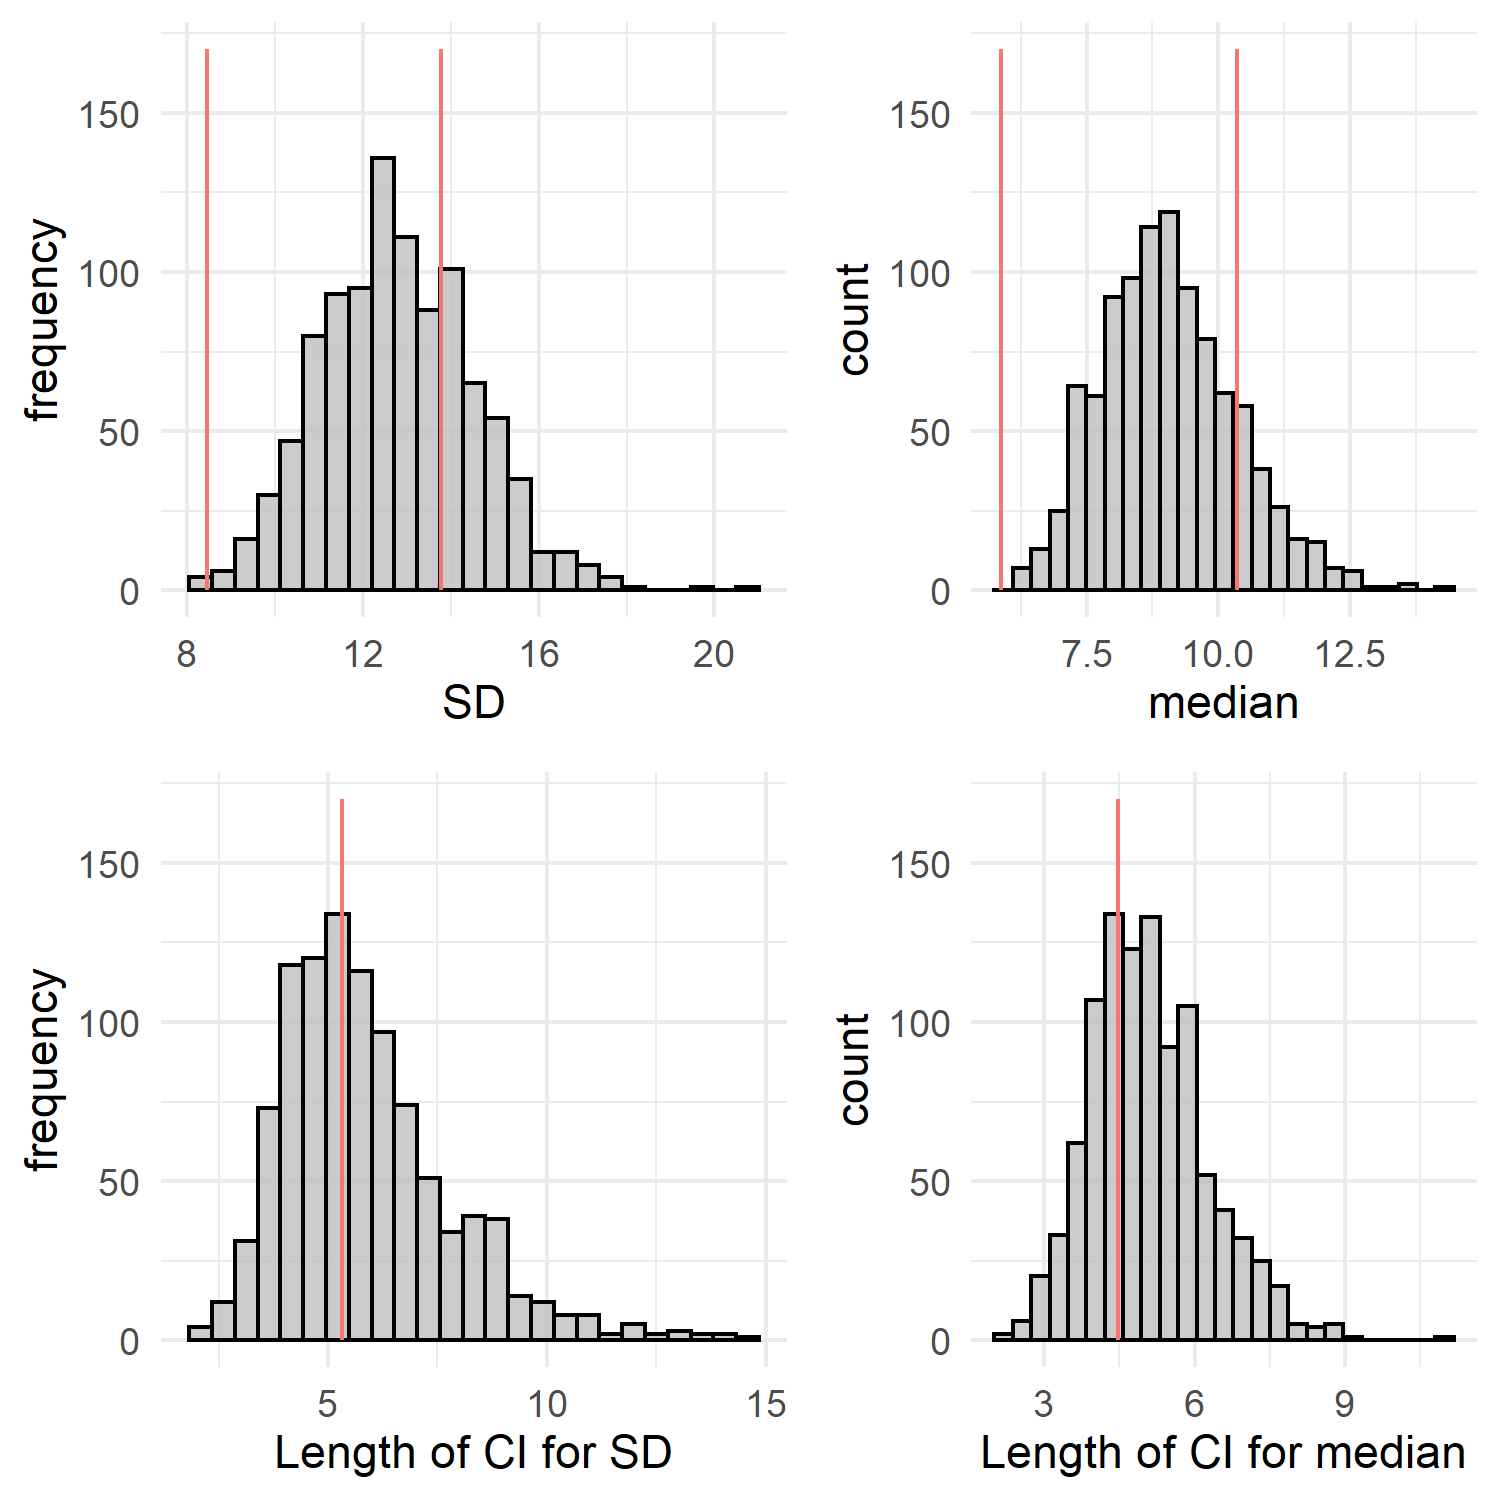
\includegraphics[width=0.8\textwidth, keepaspectratio]{ex3/MChist.png}
\caption{Histogram for 1000 MC samples of the two statistics (first row) and the length of the $95\%$ bCI (second row). The red lines show the bCI for an independent sample (first row) and the respective length (second row).}
\label{3hist}
\end{figure}  

Instead of using just the percentiles of the bootstrap distribution there is the approach of bias corrected bootstrap CIs. The function \texttt{bcanon} provided in the package \textit{bootstrap} computes an accelerated and bias-corrected bootstrap CI. A MC simulation gives good results (see last row in Table \ref{3table}) as the true statistics are always covered. The length of the CI for the median is smaller but for the SD it is greater than the ones in the first row. The mean value for the bias correction $\hat{z}_0$ is about $-0.026$ for the median and $0.124$ for the standard deviation. Taking the value of the standard normal cdf of the values shows us that on average 0.49 of the bootstrap medians are smaller than the sample median. The same holds for 0.55 of the bootstrap standard deviations respectively. On average one would expect those values close to 0.5 and thus the average $\hat{z}_0$ close to 0. The acceleration constant is computed by a transformation of the Jackknife statistics and lies at a scale of $10^{-15}$ in this case and thus is negligible. Looking at the formula this is not surprising. The median and standard deviation should not change remarkable when leaving out one instance. Especially the median ranges between at most three values anyway. Together with the small sample size of 100 the sum of distances from the Jackknife statistics' mean is not very high. Therefore we can say that the CI is constructed by taking the $\lfloor R\alpha_1 \rfloor$th and the $\lfloor R\alpha_2\rfloor$th instances of the ordered bootstrap statistics, where $\alpha_1=\Phi (z_{\alpha /2}+2\hat{z}_0)$, $\alpha_2=\Phi (z_{1-\alpha /2}+2\hat{z}_0)$ and $\Phi$ denotes the standard normal cdf. 

\section{Application for Sleep Heart Health Study data}
In this section we use the bootstrap method to build CIs for a real data set. We are just concerning the variable \texttt{rdi4p} encoding the respiratory disturbance index. The histogram (Figure \ref{3histdata}) shows the distribution of the data. As it looks like an exponential distribution (i.e. a Weibull distribution with shape parameter 1), I added the respective density with mean equal to the sample mean ($1/\lambda = 8.66$). The fit looks good and it would get better when refining the bin size, but for clearness is stay with this size.
\begin{figure}[!b]
\centering

\includegraphics[width=0.5\textwidth, keepaspectratio]{ex3/hist_data.png}
\caption{Histogram of the respiratory disturbance index (\texttt{rdi4p}) together with the density of a fitted exponential distribution (orange) with $\lambda = 0.12$.}
\label{3histdata}
\end{figure}

Now we want to estimate confidence intervals for the median and standard deviation for \texttt{rdi4p}. We use $R=1000$ bootstrap repetitions. The sample length is $n=5804$ and the sample statistics are $\hat{x}_{med}=4.19$ and $\hat{\sigma}=12.43$. The results for the percentile CI and the accelerated bias-corrected CI are shown in Table \ref{3tabledata}. We see that the function \texttt{bcanon} produced \textbf{NaN} for the CI of the median. This is because is uses the variance of the Jackknife statistics in the definition of the acceleration coefficient. As the median occurs twice in the data the denominator is zero and the acceleration coefficient is not defined. For SD we see that the upper confidence bound is smaller with the corrected method, whereas the lower bound is roughly the same as in the percentile method. It is surprising that the sample value for the standard deviation is not included in the confidence interval for the second method. The percentile CIs include both statistics. Of course, we don't know the true parameters or distribution here, so we can't judge the real precision here.  

\begin{table}[ht]
\centering
\begin{tabular}{lrrrr}
  \hline
 & lower\_med & upper\_med & lower\_sd & upper\_sd \\ 
  \hline
percentile CI & 3.95 & 4.41 & 11.80 & 13.11 \\ 
acc bias-corr CI & NaN & NaN & 11.87 & 11.95 \\ 
   \hline
\end{tabular}
\caption{Confidence intervals for median and SD using the percentile method (first row) and the accelerated bias-corrected CI using \texttt{bcanon} (second row).}
\label{3tabledata}
\end{table}
